\documentclass[11pt, a4paper]{article}
\usepackage[T2A]{fontenc}
\usepackage[utf8]{inputenc}
\usepackage[english]{babel}

%% Sets page size and margins
\usepackage[a4paper,top=3cm,bottom=3cm,left=3cm,right=3cm,marginparwidth=1.75cm]{geometry}

%% Useful packages
\usepackage{amsmath, amssymb, amsthm,calc,mathabx}
\usepackage{systeme}
\usepackage{graphicx}
\usepackage[colorinlistoftodos]{todonotes}
\usepackage[colorlinks=true, allcolors=black]{hyperref}
\usepackage{wrapfig,lipsum,booktabs}
\usepackage{enumitem}
\usepackage{float}
\usepackage{fmtcount}
\usepackage{multicol}
\usepackage{breqn}
\usepackage{setspace}
\usepackage{hyperref}
\usepackage{mathtools}
\usepackage {tikz}
	\usetikzlibrary {positioning}
	\usetikzlibrary{shapes.geometric}
\graphicspath{
	{Graphics/}
	{Graphics/BackupFunction/}
}
\newtheorem{theorem}{Theorem}

\newtheorem{lemma}{Lemma}
\newtheorem{prop}{Property}
\newtheorem*{remark}{Remark}

\theoremstyle{definition}
\newtheorem{definition}{Definition}

\setlength{\columnsep}{1cm}
\setlength{\parindent}{1em}

\newcommand\blfootnote[1]{%
	\begingroup
	\renewcommand\thefootnote{}\footnote{#1}%
	\addtocounter{footnote}{-1}%
	\endgroup
}

\begin{document}
\begin{titlepage}
	\newcommand{\HRule}{\rule{\linewidth}{0.5mm}}
	\centering
	\textsc{\LARGE Young Talents 2020}\\[1cm]
	\HRule\\[1 cm]
	{\huge\bfseries Resilient Backup Strategies}\\[0.5 cm] 
	\HRule\\
			\vfill
			\Large
			\textit{Author:}
			\textsc{Nikola Staykov}\\
            \vspace{2cm}
			\Large
			\textit{Supervisor:}
            \textsc{Yavor Papazov}\\
            
\includegraphics[width=0.5\textwidth]{Innofair_logo.png}\\
    \vfill	
	{\large\today}   
	\vfill
\end{titlepage}

\tableofcontents
\newpage
\begin{abstract}
		Backups constitute copies of data, which are to be recovered in case of need. They represent the most efficient means of precaution against ransomware attacks or natural disasters. However, they can be the source of significant costs, especially when it comes to big organizations, which keep enormous amounts of data. Therefore, backups should be carefully planned. The current project considers a theoretical model, which finds the optimal   backup strategy, consisting of full and incremental backups, considering the cost of the data recovery and storage processes. The recovery process is recreated and analyzed via Python and a Monte Carlo simulation. The model finds an optimal backup strategy given parameters, which characterize the clients' work pattern.
\end{abstract}

\section{Introduction}
	The current project builds a theoretical mathematical model in order to find an optimal backup strategy. The model considers two types of archives, full and incremental. The parameters, which we optimize, are the intervals in days between the types of archives. The structure of the archives between two full archives forms a cycle, which is then repeated indefinitely. It is defined entirely by two intervals- between two full and between two incremental backups. The results are based on two main factors, the probability of recovery failure and storage cost. The effects are calculated separately and then combined via a constant, showing the relation between the size and value of the data. Similar models have been built in the past \cite{qian2010optimal}, \cite{nakamura2003optimal}, but they consider only the storage price with non-constant generation speed. There the interval between two consecutive archives is non-constant. For the full comprehension of the project basic knowledge of probability and statistics is needed. The used definitions and notations are standard.
\newpage
\section{Theoretical setting}
		The idea behind the described model is to calculate and optimize the expected price as a sum of two components, recovery price and storage price. The two are considered separately and the expected price for each is calculated according to the backup strategy. The model combines the two via a constant, reflecting the connection between the size and value of the data. As this varies from company to company, it allows for the results to fit the user's needs.
	\subsection{Recovery}
		We will consider a backup as a structure, containing the following properties:
		$$
		B
		\begin{cases}
			d \text{: the date on which the backup was made, as a day difference from a starting point}\\
			p \text{: the probability that the recovery is unsuccessful for any reason}\\
			r \text{: the price of trying to recover the data from the given backup}
		\end{cases}
		$$
		
		Two types of backup will be considered:
		\begin{enumerate}
			\item Full backup: a backup of the whole database
			\item Incremental backup: only saves the changes from the last backup
		\end{enumerate}
		The backups from a certain type share common probability of failure and price for a recovery try.\par
		In order for an incremental backup to be successful, all the incremental backups which precede it up to a full backup need to be successful as well as the full backup itself.\par
		In this case data value should clearly be taken into account from a subjective point of view. Even though on the market some data may not be worth a lot, if it is essential for the functioning of a given company, it is clear that it will be willing to pay a lot to regain access to it immediately. Therefore, in the described model data value is considered as an ever-increasing amount, for the purposes of the research the "work rate", namely the data value generated in a day, of the company is taken as a constant. We will denote it with $w$.\par
		The cost of a backup recovery will be considered as a sum of two factors:
		\begin{itemize}
			\item The cost of redoing the lost work, denoted with $W$
			\item The cost of the recovery process itself, denoted with $R$
		\end{itemize}.
		We define $W = \Delta t.w$, where with $\Delta t$ we denote the difference in days between the successful backup and the disaster date and $R = \sum_{i=1}^{n} r_i$, where the number of attempted backups is $n$ and 
		$$
		S=\Delta t.w + R,
		$$
		Let the difference in days from the first backup to the disaster date be $T$. In case none of the backups are successful, we consider a variable $W_T$, corresponding to the price of redoing the whole work the company has done from the beginning. It is clear that $W_T>T.w$\par
\newpage
		\subsection{Storage}
		At a given moment each existing archive generates storage cost in relation to its size and the time it has existed. We assume that the size of the generated data, S, is proportional to the value of the generated data, W, described in the last paragraph. Then $Sc = W$, where $c$ is a constant. The storage price for the data generated in one day, for one day, we denote with $s$. Then the contribution to the total price of each individual archive can be described as follows:
		\begin{equation*}
			P_S = S\Delta ts
		\end{equation*}
		where with $\Delta t$ we denote the time, in which it has been kept.\\
		Full and incremental backups have different contribution as the size of full backups is constantly growing and the size of incremental backups is fixed.
	\section{Recovery price}
		This section describes the component of the model, related to the recovery process and the following re-make of lost data.
		\subsection{Full backups only}
		When we only consider a set of full backups, the model is simply a Bernoulli distribution with finite trials, namely the number of full backups. We stop when we find a successful backup, starting from the latest and going to the last. Let us define the properties of a full backup($B_F$):
		$$
		B_F
		\begin{cases}
			p_F: \text{the probability of failure}\\
			r_F: \text{the recovery trial cost}\\
			t_F: \text{the days between two consecutive full backups}\\
		\end{cases}
		$$
		Let $k$ be the number of full backups made before the disaster date. Then:
		$$
			k = \left \lfloor{\frac{T}{t_F}}\right \rfloor + 1
		$$
		We can now define the expected backup cost:
		\begin{equation}
		\label{eq:1}
			E(T) = p_F^{k}\left(W_T + k.r_F\right) + \displaystyle \sum_{i=0}^{k-1} (1-p_F).p_F^{i}\left( \left (\left\{ \frac{T}{t_F}\right \} + i\right)t_F.w + (i+1).r_F \right )
		\end{equation}
		This calculation is essential as incremental backups can only work when there is a working full backup and therefore the first thing we need to do is find the latest one. We can now move on to considering the incremental backups given a working full backup.
		\subsection{Incremental backups with a working full backup}
		We will now consider the case when we have a working backup and we are trying to recover additional data from the incremental backups.\\
		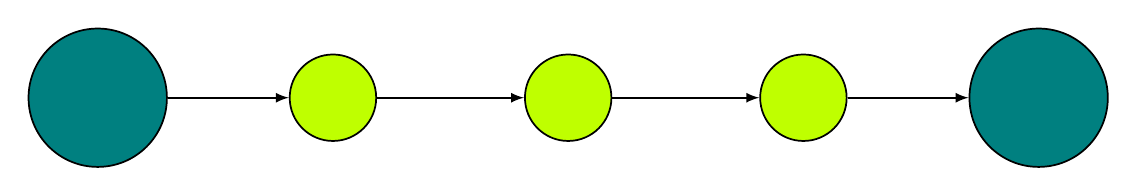
\begin{tikzpicture}
		[every node/.style={inner sep=0pt}]
		\node (1) [circle, minimum size=50.0pt, fill=teal, line width=0.625pt, draw=black] at (50.0pt, -130pt)  {};
		\node (2) [circle, minimum size=31.25pt, fill=lime, line width=0.625pt, draw=black] at (135pt, -130pt)  {};
		\node (3) [circle, minimum size=31.25pt, fill=lime, line width=0.625pt, draw=black] at (220pt, -130pt)  {};
		\node (4) [circle, minimum size=31.25pt, fill=lime, line width=0.625pt, draw=black] at (305pt, -130pt)  {};
		\node (5) [circle, minimum size=50.0pt, fill=teal, line width=0.625pt, draw=black] at (390pt, -130pt)  {};
		\draw [line width=0.625, ->, >=latex, color=black] (1) to  (2);
		\draw [line width=0.625, ->, >=latex, color=black] (2) to  (3);
		\draw [line width=0.625, ->, >=latex, color=black] (3) to  (4);
		\draw [line width=0.625, ->, >=latex, color=black] (4) to  (5);
		\end{tikzpicture}\\
		Let	us define the the properties of the incremental backup($B_I$) in a similar fashion:
		$$
		B_I
		\begin{cases}
			p_I: \text{the probability of failure}\\
			r_I: \text{the recovery trial cost}\\
			t_I: \text{the days between two consecutive incremental backups}\\
		\end{cases}
		$$
\newpage
		Let $T_F$ denote the difference in days between the disaster date and the successful full backup and $l$ denote the number of incremental backups we have to consider. We have two options for $l$ depending on whether the latest full backup was successful:
		$$
			l=
			\begin{cases}
				\left\lfloor \frac{T_F}{t_I}\right \rfloor \text{, if } T_F<t_F\\
				\left\lfloor \frac{t_F}{t_I}\right \rfloor -1 \text{, if } T_F>t_F\footnotemark\\
			\end{cases}
		$$
		\footnotetext{We can only try to recover incremental backups preceding the next full backup}
		Note that the last full backup being successful is equivalent to $T_F<t_F$.\par
		We are in the exact opposite situation with respect to the previous subsection. The process of recovering incremental backups continues until we conduct an unsuccessful attempt to recover the data, as this will mean none of the following backups can be used either. Note that we are reducing $W$ since in the initial position we are willing to redo the work up to the working full backup. That being said, we are ready to calculate the expected price:
		\begin{equation}
		\label{eq:2}
			f(T_F) = (1-p_I)^l.((T_F-t_I.l).w + r_I.l) + \displaystyle \sum_{i=0}^{l-1} (1-p_I)^{i}.p_I((T_F-t_I.i)w + r_I.(i+1))
		\end{equation}
		Now we know how much the price will decrease when we use incremental backups and can build the whole picture using equations \ref{eq:1} and \ref{eq:2}.
		\subsection{Overall expected price}
		For each summand in \ref{eq:1} we should add the effect of incremental backups, so we get new summands of the type:
		$$
		P(W + R),
		$$
		where $P$ is the probability of a certain combination of events occurring, $W$ is the cost of the data that has to be reworked and $R$ is the cost of the recovery process. Incremental backups lower the cost of the data that has to be reworked but make $R$ bigger. As mentioned before, there is only one case when the number of incremental backups we have to consider is different and it corresponds to the first full backup being successful. If the $i$-th full backup is successful\footnote{This corresponds to the $i-1$-th summand in the sum from equation \ref{eq:3}}:
		$$
		T_F=t_F\left(\left\{ \frac{T}{t_F} \right\} + i - 1\right)
		$$
		By combining equations \ref{eq:1} and \ref{eq:2} we get:
		\begin{equation}\label{eq:3}
			F(T) = p_F^{k}(W_T+k.r_F) + \displaystyle\sum_{i=0}^{k-1}(1-p_F).p_F^{i}\left(f(T_F) + (i+1).r_F\right)
		\end{equation}
		Using the described equations \ref{eq:1} and \ref{eq:3}, we can construct a graph of the expected price with and without incremental backups included.
		\begin{figure}[H]
			\begin{minipage}{1.0\textwidth}
				\centering
				\includegraphics[width=0.7\textwidth]{"Weekly_full"}
				\caption{Full only and Whole model}\label{Fig:FullWeekly}
			\end{minipage}
		\end{figure}
		\subsection{Correlation of data}
		\subsection{Monte Carlo simulation}
			A Monte Carlo simulation has been build with python to generate random recovery processes with the described conditions of backup structure. The price of the recovery has been graphed with respect to the disaster date:
			\begin{figure}[H]
				\begin{minipage}{1.0\textwidth}
					\centering
					\includegraphics[width=0.7\textwidth]{"Weekly_full_carlo"}
					\caption{Monte Carlo simulation}\label{Fig:MonteCarlo}
				\end{minipage}
			\end{figure}
		\blfootnote{In both Figure \ref{Fig:FullWeekly} and Figure \ref{Fig:MonteCarlo} the data showed is for a weekly full and daily incremental backups}
		The colors in Figure \ref{Fig:MonteCarlo} represent the type of the last backup, which was successful during the recovery, full, incremental or non-existing.
		\newpage
		A linear regression has been made of the data generated, which is to show that the effect of initial unsecured data fades with time, as the price of failure is calculated as the price to redo the whole work from the creation of the company.
\section{Storage price}
	The storage price is generated from the existing archives as for each individually depends on its type and creation dates. For the purposes of the model we assume that the size of the data, S, is proportional to the price of their creation. We introduce the constant $c=\dfrac{S}{W}$.\\
	At a given moment, T, we want to calculate the the contribution of a full backup, created $d$ days after the first backup. The number of days of generating data before the first archive we will denote with $T_0$. Then the archive has size $S=\dfrac{W}{c}=\dfrac{w\Delta t}{c}=\dfrac{w}{c}(T_0 + d)$, where $w$ is the work rate from the previous component. The storage price for a day is $s=\dfrac{w}{c}$ and we have kept it $T-d$ days. Therefor the backup has generated storage price:
	$$
	\dfrac{w}{c}(T_0 + d)s(T-d).
	$$
	Incremental backups, on the other hand, have fixed size $cwt_I$. Their contribution to the storage price is only change by the time they have been kept, namely $T-d$. Therefore the contribution of an incremental archive, created $d$ days after the first backup is:
	$$
	\dfrac{w}{c}t_Is(T-d)
	$$
	Let $B_I$ be the set of all incremental backups and $B_F$ that of all full backups. The the storage price is:
	\begin{equation}\label{eq:4}
		\left(\displaystyle\sum_{b\in B_F}\dfrac{w^2}{c^2}(T_0 + d_b)(T-d_b)\right) + 	\left(\displaystyle\sum_{b\in B_I}\dfrac{w^2}{c^2}t_I(T-d_b)\right).
	\end{equation}
	For $b\in B_F$, $d_b$ takes values:
	$$lt_F|\ l\in \left[0,\left\lfloor\dfrac{T}{t_F}\right\rfloor t_F\right],$$
	and for $b\in  B_I$:
	$$d_b= mt_F + nt_I|\ m\in \left[0, \left\lfloor\dfrac{T}{t_F}\right\rfloor\right],n\in \left[1, \left\lfloor\dfrac{t_F}{t_I}\right\rfloor\right].$$
	Substituting in \ref{eq:4} we get
	\begin{equation}
		\left(\displaystyle\sum_{l = 0}^{\left\lfloor\frac{T}{t_F}\right\rfloor t_F}\dfrac{w^2}{c^2}(T_0 + lt_F)(T-lt_F)\right) + \left(\displaystyle\sum_{m = 0}^{\left\lfloor\frac{T}{t_F}\right\rfloor}\displaystyle\sum_{n = 1}^{\left\lfloor\frac{t_F}{t_I}\right\rfloor}\dfrac{w^2}{c^2}t_I(T-mt_F + nt_I)\right)
	\end{equation}
	With that we ca find the storage price of the generated data. Changing the ratio between the storage size and the value of the generated data ($c$), we can find optimal backup strategies with respect to the intervals between consecutive full and incremental backups.
\section{Results}
	The table below summarizes the results for an optimal strategy for different values of $c$:
	\begin{center}
		\begin{tabular}{| l | l | l |}
			\hline
			Constant $c$ & Full interval & Incremental interval\\ \hline
			100-200 & 29 & 16\\ \hline
			200-400 & 29 & 10\\ \hline
			400-600 & 21 & 8\\ \hline
			600-800 & 16 & 6\\ \hline
			800-1000 & 16 & 6\\ \hline
			1000-1400 & 13 & 5\\ \hline
			1400-1600 & 11 & 3\\ \hline
			1600-4100 & 8 & 3\\ \hline
			4100-4500 & 6 & 3\\ \hline
			4500-7000 & 5 & 2\\ \hline
		\end{tabular}
	\end{center}
	\begin{figure}[H]
		\begin{minipage}{1.0\textwidth}
			\centering
			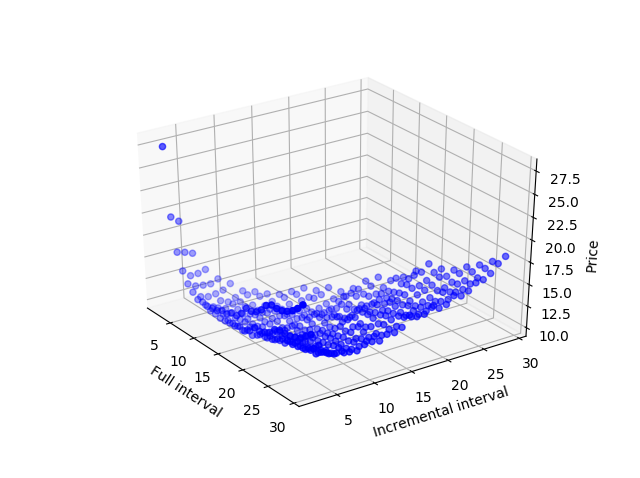
\includegraphics[width=0.7\textwidth]{3d_all_1.png}
			\caption{Visualization for $c=1000$}\label{Fig:Whole_model}
		\end{minipage}
	\end{figure}
	\newpage
\section{Further development}
	The author considers several future development directions for the project, namely:
	\begin{itemize}
		\item non-constant work rate for the 
		\item complex connection between data value and storage price
		\item Data correlation for easier recovery from partial leftover files
	\end{itemize}
\section{Acknowledgments}
I want to thank my mentor, Yavor Papazov, and Konstantin Delchev for the enormous help with the choice of the research subject and for providing me with all the necessary material to get familiar with the topic, as well as listening to my questions along the whole way. I extend my gratitude towards HSSIMI and SRS for the opportunity to develop this project and the irreplaceable atmosphere of dedication and concentration.
\bibliographystyle{unsrt}
\nocite{*}
\bibliography{Bibliography}
\end{document}